\begin{figure}
\centering
\begin{subfloat}[]{
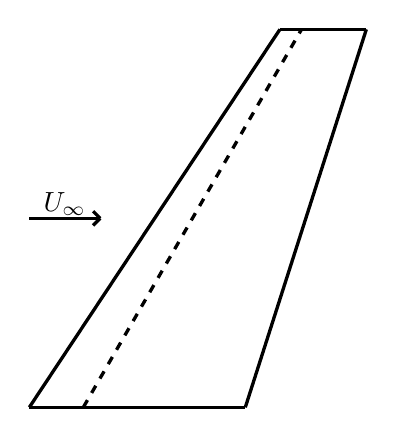
\begin{tikzpicture}[scale=0.3,auto = left,
measure/.style = {very thin,
        {Bar[width=2.2mm]Straight Barb[]}-%
        {Straight Barb[]Bar[width=2.2mm]},
            },
every label/.append style = {font=\footnotesize}]

        \coordinate (LE_R) at ( 0, 0, 0 );
        \coordinate (TE_R) at ( 9.1428, 0, 0 );
        \coordinate (LE_T) at ( 10.609, 16, 0 );
        \coordinate (TE_T) at ( 14.266, 16, 0 );
        \draw[very thick,black] (LE_R) -- (TE_R);
        \draw[very thick,black] (LE_T) -- (TE_T);
        \draw[very thick,black] (LE_T) -- (LE_R);
        \draw[very thick,black] (TE_R) -- (TE_T);
        \coordinate (AC_R) at ( 2.2857, 0, 0 );
        \coordinate (AC_T) at ( 11.52325, 16, 0 );
        \draw[very thick,black,dashed] (AC_R) -- (AC_T);

        
        \coordinate (UInf_Start) at ( 0, 8, 0 );
        \coordinate (UInf_End) at ( 3, 8, 0 );
        \coordinate (UInf_End_ArrUp) at ( 2.7, 8.3, 0 );
        \coordinate (UInf_End_ArrDown) at ( 2.7, 7.7, 0 );
        \coordinate (UInf_Text) at ( 1.5, 8.6, 0 );
        \draw[very thick,black] (UInf_Start) -- (UInf_End);
        \draw[very thick,black] (UInf_End_ArrUp) -- (UInf_End);
        \draw[very thick,black] (UInf_End_ArrDown) -- (UInf_End);
        \node [] at (UInf_Text) {$U_\infty$}; 
        
    \end{tikzpicture}
}
\end{subfloat}
\hspace{1cm}
\begin{subfloat}[]{
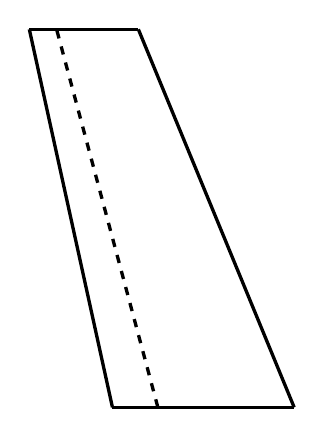
\begin{tikzpicture}[scale=0.3,auto = left,
measure/.style = {very thin,
        {Bar[width=2.2mm]Straight Barb[]}-%
        {Straight Barb[]Bar[width=2.2mm]},
            },
every label/.append style = {font=\footnotesize}]

        \coordinate (LE_R) at ( 0, 0, 0 );
        \coordinate (TE_R) at ( 7.692, 0, 0 );
        \coordinate (LE_T) at ( -3.518, 16, 0 );
        \coordinate (TE_T) at ( 1.0974, 16, 0 );
        \draw[very thick,black] (LE_R) -- (TE_R);
        \draw[very thick,black] (LE_T) -- (TE_T);
        \draw[very thick,black] (LE_T) -- (LE_R);
        \draw[very thick,black] (TE_R) -- (TE_T);
        
        \coordinate (AC_R) at ( 1.923, 0, 0 );
        \coordinate (AC_T) at ( -2.36415, 16, 0 );
        \draw[very thick,black,dashed] (AC_R) -- (AC_T);
        
    \end{tikzpicture}
    }
\end{subfloat}
\caption[Visual representation of investigated geometries]{Visual representation of the investigated geometries \cite{rausa2026monnalisa}: \textbf{(a)} first and \textbf{(b)} second geometry. The dashed line represents the aerodynamic center line that defines the sweep angle.}
\label{fig:AllGeometries}
\end{figure}